% =============================================================================
% FIGURE CAPTIONS FOR MASS SPECTROMETRY AND DROPLET ENCODING FIGURES
% =============================================================================
% Author: Kundai Sachikonye
% These captions are designed for large multi-panel figures that require
% detailed explanations of each subpanel.
% =============================================================================

% -----------------------------------------------------------------------------
% FIGURE 1: TIME-OF-FLIGHT MASS SPECTROMETER
% -----------------------------------------------------------------------------
\begin{figure}[htbp]
    \centering
    \includegraphics[width=\textwidth]{figures/01_tof_mass_spectrometer.png}
    \caption{\textbf{Time-of-Flight (TOF) Mass Spectrometer: Ion trajectory dynamics and detection principles.}
    (\textbf{A}) 3D Ion Trajectories demonstrating mass-dependent flight paths through the TOF analyzer. Lighter ions (m/z = 100, blue) arrive at the detector before heavier ions (m/z = 500, green; m/z = 1000, orange; m/z = 2000, red), with flight times proportional to $\sqrt{m/z}$. Trajectories show minimal spatial dispersion ($\pm$0.04 mm) in the radial dimension, confirming effective ion beam collimation. The vertical axis spans 0--1000 arbitrary units representing detector position.
    (\textbf{B}) Velocity-Time Relationship showing the fundamental TOF equation $v = \sqrt{2eV/m}$ across the m/z range 150--2000 and flight times 2.5--20 $\mu$s. The 3D surface illustrates how ion velocity (300--1000 m/s) depends inversely on mass, with the color gradient (purple to yellow) indicating velocity magnitude. This relationship enables mass determination from measured arrival times with sub-ppm precision at high resolution.
    (\textbf{C}) Energy Distribution Phase Space demonstrating reflectron focusing for energy compensation. The 3D surface shows angular spread (0--12$^\circ$) as a function of initial position (0--100 mm) and kinetic energy (0--100 eV). Reflectron geometry creates a focal plane where ions of identical m/z but different initial energies arrive simultaneously, improving mass resolution from $\sim$5,000 to $>$40,000 FWHM.
    (\textbf{D}) Detection Efficiency Landscape mapping microchannel plate (MCP) response across impact angle (0--100$^\circ$) and m/z (0--8000). Detection efficiency (0--0.8) peaks at normal incidence and decreases with increasing mass due to reduced secondary electron yield. The 3D surface guides optimal detector positioning and predicts sensitivity variations across the mass range.}
    \label{fig:tof_mass_spectrometer}
\end{figure}

% -----------------------------------------------------------------------------
% FIGURE 2: QUADRUPOLE MASS FILTER
% -----------------------------------------------------------------------------
\begin{figure}[htbp]
    \centering
    \includegraphics[width=\textwidth]{figures/02_quadrupole_mass_filter.png}
    \caption{\textbf{Quadrupole Mass Filter: RF trajectory dynamics and mass-selective transmission.}
    (\textbf{A}) 3D RF Trajectory Dynamics comparing stable (transmitted, green helix) and unstable (rejected, red expanding spiral) ion trajectories. Stable ions execute bounded oscillations within the quadrupole field ($\pm$4 mm radial extent) over multiple RF cycles (0--50), while unstable ions exhibit exponentially growing amplitudes leading to electrode collision. The helical trajectory pattern reflects the superposition of secular motion at frequency $\omega_0$ and RF micromotion at $\Omega$.
    (\textbf{B}) Mathieu Stability Diagram showing the first stability region in $(a, q)$ parameter space, where $a = 8eU/m\Omega^2 r_0^2$ and $q = 4eV/m\Omega^2 r_0^2$. The 3D surface displays transmission probability (0--1.0) across the stability zone bounded by $\beta_x = 0, 1$ and $\beta_y = 0, 1$ iso-lines. Only ions within the stable region (green/yellow) reach the detector; operating at the apex provides unit mass resolution while the base enables high transmission.
    (\textbf{C}) Potential Energy Landscape illustrating the saddle-point potential $\Phi(x,y) = \frac{\Phi_0}{r_0^2}(x^2 - y^2)$ characteristic of quadrupole fields. The 3D surface spans $\pm$4 mm in both transverse dimensions with potential ranging from $-$750 to $+$750 V. The hyperbolic saddle shape creates focusing in one plane and defocusing in the orthogonal plane, with RF alternation producing net confinement for stable masses.
    (\textbf{D}) Mass Scan Performance showing the speed-sensitivity trade-off across scan rates (100--1000 amu/s) and target m/z (0--2000). The 3D surface displays peak intensity (0--900 counts) degradation at high scan speeds due to insufficient ion transit time for stable trajectory establishment. Optimal operation balances throughput against resolution requirements, with the color gradient indicating sensitivity from purple (low) to yellow (high).}
    \label{fig:quadrupole_mass_filter}
\end{figure}

% -----------------------------------------------------------------------------
% FIGURE 3: ION TRAP (PAUL TRAP)
% -----------------------------------------------------------------------------
\begin{figure*}[!htbp]
    \centering
    \includegraphics[width=\textwidth]{03_paul_trap.png}
    \caption{\textbf{Ion Trap (Paul Trap): 3D confinement dynamics and mass-selective ejection mechanisms.}
    (\textbf{A}) 3D Trapping Trajectories showing complex Lissajous patterns within the trap volume. Ion motion exhibits quasi-periodic oscillations in radial ($\pm$2 mm) and axial ($\pm$3 mm) dimensions over multiple RF cycles. Color-coded trajectories (purple to yellow gradient) demonstrate secular motion with frequencies $\omega_r$ and $\omega_z$ creating intricate 3D orbital patterns. Bounded trajectories confirm stable trapping with ions confined within the yellow boundary surface representing the trap's effective potential well.
    (\textbf{B}) Effective Potential Wells demonstrating harmonic confinement with pseudopotential $U_{\text{eff}}(r,z) = \frac{1}{2}m(\omega_r^{2} r^{2} + \omega_z^{2} z^{2})$. The 3D surface shows radial (0--5 mm) and axial ($\pm$4 mm) potential distribution with energy scale 0--70,000 eV. Deep potential wells (purple regions) provide strong ion confinement, while the harmonic shape enables mass-dependent secular frequencies. Color gradient from purple (deep well) to yellow (high potential) illustrates the three-dimensional trapping geometry.
    (\textbf{C}) Mass Ejection Dynamics showing resonance ejection mechanism across m/z range 0--1000. The 3D surface demonstrates ejection time (0--10 ms) dependence on applied ejection voltage (0--10 V) and target mass. Parametric resonance excitation selectively destabilizes specific m/z values, with ejection time decreasing at higher voltages. Color progression from purple (long ejection times) to yellow (rapid ejection) shows mass-selective scanning capability through controlled resonance activation.
    (\textbf{D}) Ion Cloud Evolution demonstrating collisional cooling effects over time (0--10 ms). Three temporal snapshots show ion density distribution across the trap cross-section ($\pm$4 mm $\times$ $\pm$4 mm). Initial broad distribution (top layer) progressively contracts through buffer gas collisions, reaching thermal equilibrium (bottom layer). Color scale from purple (low density) to yellow (high density) illustrates spatial compression and temperature reduction, improving mass resolution by reducing ion kinetic energy spread.}
    \label{fig:paul_trap}
\end{figure*}

% -----------------------------------------------------------------------------
% FIGURE 4: FT-ICR MASS SPECTROMETER
% -----------------------------------------------------------------------------
\begin{figure}[htbp]
    \centering
    \includegraphics[width=\textwidth]{04_fticr_mass_spectrometer.png}
    \caption{\textbf{FT-ICR (Fourier Transform Ion Cyclotron Resonance) Mass Spectrometer: Cyclotron motion and frequency-based mass measurement.}
    (\textbf{A}) 3D Ion Cyclotron Orbits demonstrating mass-dependent orbital frequencies in a 7 Tesla magnetic field. Ions execute circular orbits in the $xy$-plane perpendicular to the magnetic field vector $\mathbf{B}$ (indicated by arrow), with cyclotron frequency $\omega_c = qB/m$ inversely proportional to mass. Lighter ions (m/z = 100, red) complete more orbits per unit time than heavier ions (m/z = 500, blue; m/z = 1000, green; m/z = 2000, purple). The slight axial drift along $z$ reflects magnetron motion and ion injection dynamics. Orbital radius remains constant ($\sim$30 mm) for ions of equal kinetic energy.
    (\textbf{B}) Cyclotron Frequency Relationship showing the fundamental FT-ICR equation $\omega_c = qB/m$ as a 3D surface across m/z range 0--2000 and magnetic field strength 4--14 Tesla. Cyclotron frequency (0.25--1.75 MHz) decreases with increasing mass and increases with magnetic field strength. The surface gradient illustrates why higher magnetic fields provide better mass resolution: frequency separation $\Delta\omega_c$ between adjacent masses scales linearly with $B$. Color gradient from purple (low frequency) to yellow (high frequency) enables rapid visual assessment of operating conditions.
    (\textbf{C}) Image Current Detection illustrating the Fourier Transform process that converts time-domain ion signals to mass spectra. The 3D visualization shows: time-domain transient signal (blue oscillating trace in $xz$-plane) representing image current induced by orbiting ion packets, and frequency-domain peaks (red bars in $yz$-plane) obtained via FFT. Multiple m/z components (500, 750, 1000) produce distinct frequency peaks that are resolved and converted to mass values. Signal decay reflects ion dephasing and collision-induced damping over the 0--1000 ms acquisition window.
    (\textbf{D}) Mass Resolution Landscape showing the ultra-high resolution capability of FT-ICR across m/z range 0--2000 and observation time 0--2 seconds. Resolution $R = m/\Delta m$ exceeds $10^6$ at low mass with extended transient times, following $R \propto \omega_c \cdot T_{\text{obs}}$. The 3D surface (purple to yellow gradient) demonstrates that resolution degrades with increasing mass (lower $\omega_c$) but improves with longer observation times. This trade-off between throughput and resolution guides experimental design for ultrahigh-resolution applications including isotope fine structure and isobaric separation.}
    \label{fig:fticr_mass_spectrometer}
\end{figure}

% -----------------------------------------------------------------------------
% FIGURE 5: ORBITRAP MASS SPECTROMETER
% -----------------------------------------------------------------------------
\begin{figure*}[!htbp]
    \centering
    \includegraphics[width=\textwidth]{05_orbitrap_mass_spectrometer.png}
    \caption{\textbf{Orbitrap Mass Spectrometer: Electrostatic trapping and axial oscillation frequency detection.}
    (\textbf{A}) 3D Ion Trajectories in Orbitrap showing the characteristic spiral motion around the central spindle electrode (gray surface). Ions are injected tangentially and orbit the central electrode while oscillating axially with frequency $\omega = \sqrt{k/m}$, where $k$ is the field curvature constant. Different m/z values (200 red, 500 blue, 1000 green, 1500 purple) exhibit mass-dependent axial frequencies: lighter ions oscillate faster, completing more $z$-axis cycles during a single orbital period. The spindle electrode geometry (hyperboloid shape) generates the quadro-logarithmic potential that provides harmonic axial restoring force while maintaining stable radial orbits ($\pm$20--50 mm radius).
    (\textbf{B}) Axial Oscillation Frequency showing the fundamental Orbitrap equation $\omega = \sqrt{k/m}$ as a 3D surface across m/z range 100--2000 and relative field strength 0.5--2.0. Axial frequency (1--5 kHz typical) decreases with $\sqrt{m}$ and increases with field strength. Unlike FT-ICR where $\omega_c \propto 1/m$, the Orbitrap's $\omega \propto 1/\sqrt{m}$ dependence provides more uniform frequency spacing across the mass range. Color gradient (purple to yellow) indicates frequency magnitude, with highest frequencies at low mass and high field strength.
    (\textbf{C}) Orbitrap Electrostatic Potential displaying the quadro-logarithmic field $U(r,z) = \frac{k}{2}\left(z^2 - \frac{r^2}{2}\right) + \frac{k}{2}R_m^2\ln(r/R_m)$ characteristic of the Orbitrap geometry. The 3D surface shows potential (normalized 0--1) as a function of radial position $r$ (10--50 mm) and axial position $z$ ($\pm$40 mm). The saddle-point topology provides axial confinement (harmonic well along $z$) while permitting stable radial orbits (logarithmic potential in $r$). Contour lines on the $z = 0$ plane illustrate equipotential surfaces. The central electrode radius $R_m \approx$ 8 mm defines the inner boundary.
    (\textbf{D}) Orbitrap Resolution showing mass resolving power $R = m/\Delta m$ as a function of m/z (200--2000) and transient acquisition time (32--512 ms). Resolution scales as $R \propto \omega \cdot T_{\text{transient}} \propto T/\sqrt{m}$, reaching 240,000 at m/z 400 with 256 ms transient (marked with red star as typical operating point). The 3D surface (purple to yellow gradient) demonstrates the resolution-speed trade-off: shorter transients enable faster scan rates at reduced resolution, while extended transients achieve ultrahigh resolution for applications requiring isotopic fine structure or isobaric discrimination. Maximum resolution exceeds 500,000 at low mass with 512 ms transients.}
    \label{fig:orbitrap_mass_spectrometer}
\end{figure*}

% -----------------------------------------------------------------------------
% FIGURE 6: CATEGORICAL STATE SYNTHESIZER
% -----------------------------------------------------------------------------
\begin{figure*}[!htbp]
    \centering
    \includegraphics[width=\textwidth]{10_categorical_synthesizer.png}
    \caption{\textbf{Categorical State Synthesizer: Inverse measurement for molecular state design.}
    (\textbf{A}) Specify Target State showing the S-Entropy coordinate specification interface. The 3D visualization displays the target state (red star) at coordinates $(S_k, S_t, S_e) = (0.7, 0.5, 0.8)$ within the unit cube $[0,1]^3$. The blue shaded region represents the reachable state space constrained by physical realizability bounds. Users specify desired molecular properties through S-Entropy coordinates rather than explicit molecular structure, enabling inverse design from observables.
    (\textbf{B}) Determine Conditions showing the input filter that computes required experimental conditions from target S-Entropy coordinates. For target $(0.7, 0.5, 0.8)$, the system determines: Temperature = 298 K, Pressure = 1 atm, Field = 50 mV/m, Frequency = 2.4 GHz, Gradient = 15\%/cm. Physical constraints are automatically enforced: thermodynamically stable (green check), within realizability bounds (green check), no forbidden transitions (green check).
    (\textbf{C}) Generate Protocol showing the output filter that produces an executable synthesis protocol. The step-by-step procedure includes: (1) Initialize system and equilibrate to 298 K, (2) Drive vibrational modes at specified frequencies (2.35 GHz for 10 ms, 2.47 GHz for 15 ms, 2.68 GHz for 8 ms), (3) Apply field gradient 15\%/cm for 20 minutes while monitoring S-coordinates, (4) Verify convergence within 5\% of target. Duration estimates and success probabilities are provided.
    (\textbf{D}) Synthesis Trajectory showing convergence from initial to target state. The plot tracks S-Entropy coordinates ($S_k$ blue, $S_t$ red, $S_e$ green) as functions of synthesis progress (0--1). All three coordinates monotonically approach their target values (dashed lines at 0.7, 0.5, 0.8), demonstrating successful state synthesis through the categorical framework. Convergence is achieved at progress = 0.95 within specified tolerances.}
    \label{fig:categorical_synthesizer}
\end{figure*}

% -----------------------------------------------------------------------------
% FIGURE 5: VIRTUAL DETECTOR MULTIMODAL
% -----------------------------------------------------------------------------
\begin{figure*}[htbp]
    \centering
    \includegraphics[width=\textwidth]{14_virtual_detector_multimodal.png}
    \caption{\textbf{Virtual Detector Multimodal: Same ion measured across four virtual instrument platforms.}
    Test ion: m/z 659.8, RT 12.3 min, Intensity $1 \times 10^5$.
    (\textbf{Column A}) 3D Spectrum Views showing mass spectral peaks for qTOF (top), Virtual TOF (second), Virtual Orbitrap (third), and Virtual FT-ICR (bottom). Each platform produces characteristic peak shapes: qTOF shows broad Gaussian profiles, TOF exhibits symmetric peaks, Orbitrap displays narrow symmetric peaks, and FT-ICR produces the sharpest peaks reflecting ultrahigh resolution. The m/z axis spans 0--1000 with intensity scaling to $1 \times 10^5$.
    (\textbf{Column B}) Measurable Properties listing ion characteristics extracted by each virtual instrument. All platforms correctly identify m/z = 659.8000 (measured values: qTOF 659.8000, TOF 659.8048, Orbitrap 659.7906, FT-ICR 659.8048) with platform-specific precision. Additional properties include charge state, isotope patterns (M+1, M+2 ratios), retention time (12.3 min), peak width (FWHM varying from 0.1 Da for qTOF to 0.001 Da for FT-ICR), and categorical state classification.
    (\textbf{Column C}) Performance Metrics comparing platform capabilities via horizontal bar charts. Metrics include: Dynamic Range (0.43--0.79), Sensitivity (0.76--0.86), Resolution (0.00--1.00), and Mass Accuracy (0.76--1.00). FT-ICR achieves maximum resolution (1.00) and mass accuracy (1.00), while qTOF provides balanced performance across all metrics.
    (\textbf{Column D}) CV Validation Droplet Analysis showing thermodynamic droplet wave patterns generated from each platform's measurement. Concentric ring patterns with green ``CV Passed'' indicators confirm successful computer vision validation. The droplet morphology (ring spacing, amplitude decay) encodes the same underlying ion identity despite platform-specific measurement characteristics, demonstrating cross-platform consistency.}
    \label{fig:virtual_detector_multimodal}
\end{figure*}

% -----------------------------------------------------------------------------
% FIGURE 6: VIRTUAL DETECTOR CV ENHANCED
% -----------------------------------------------------------------------------
\begin{figure*}[!htbp]
    \centering
    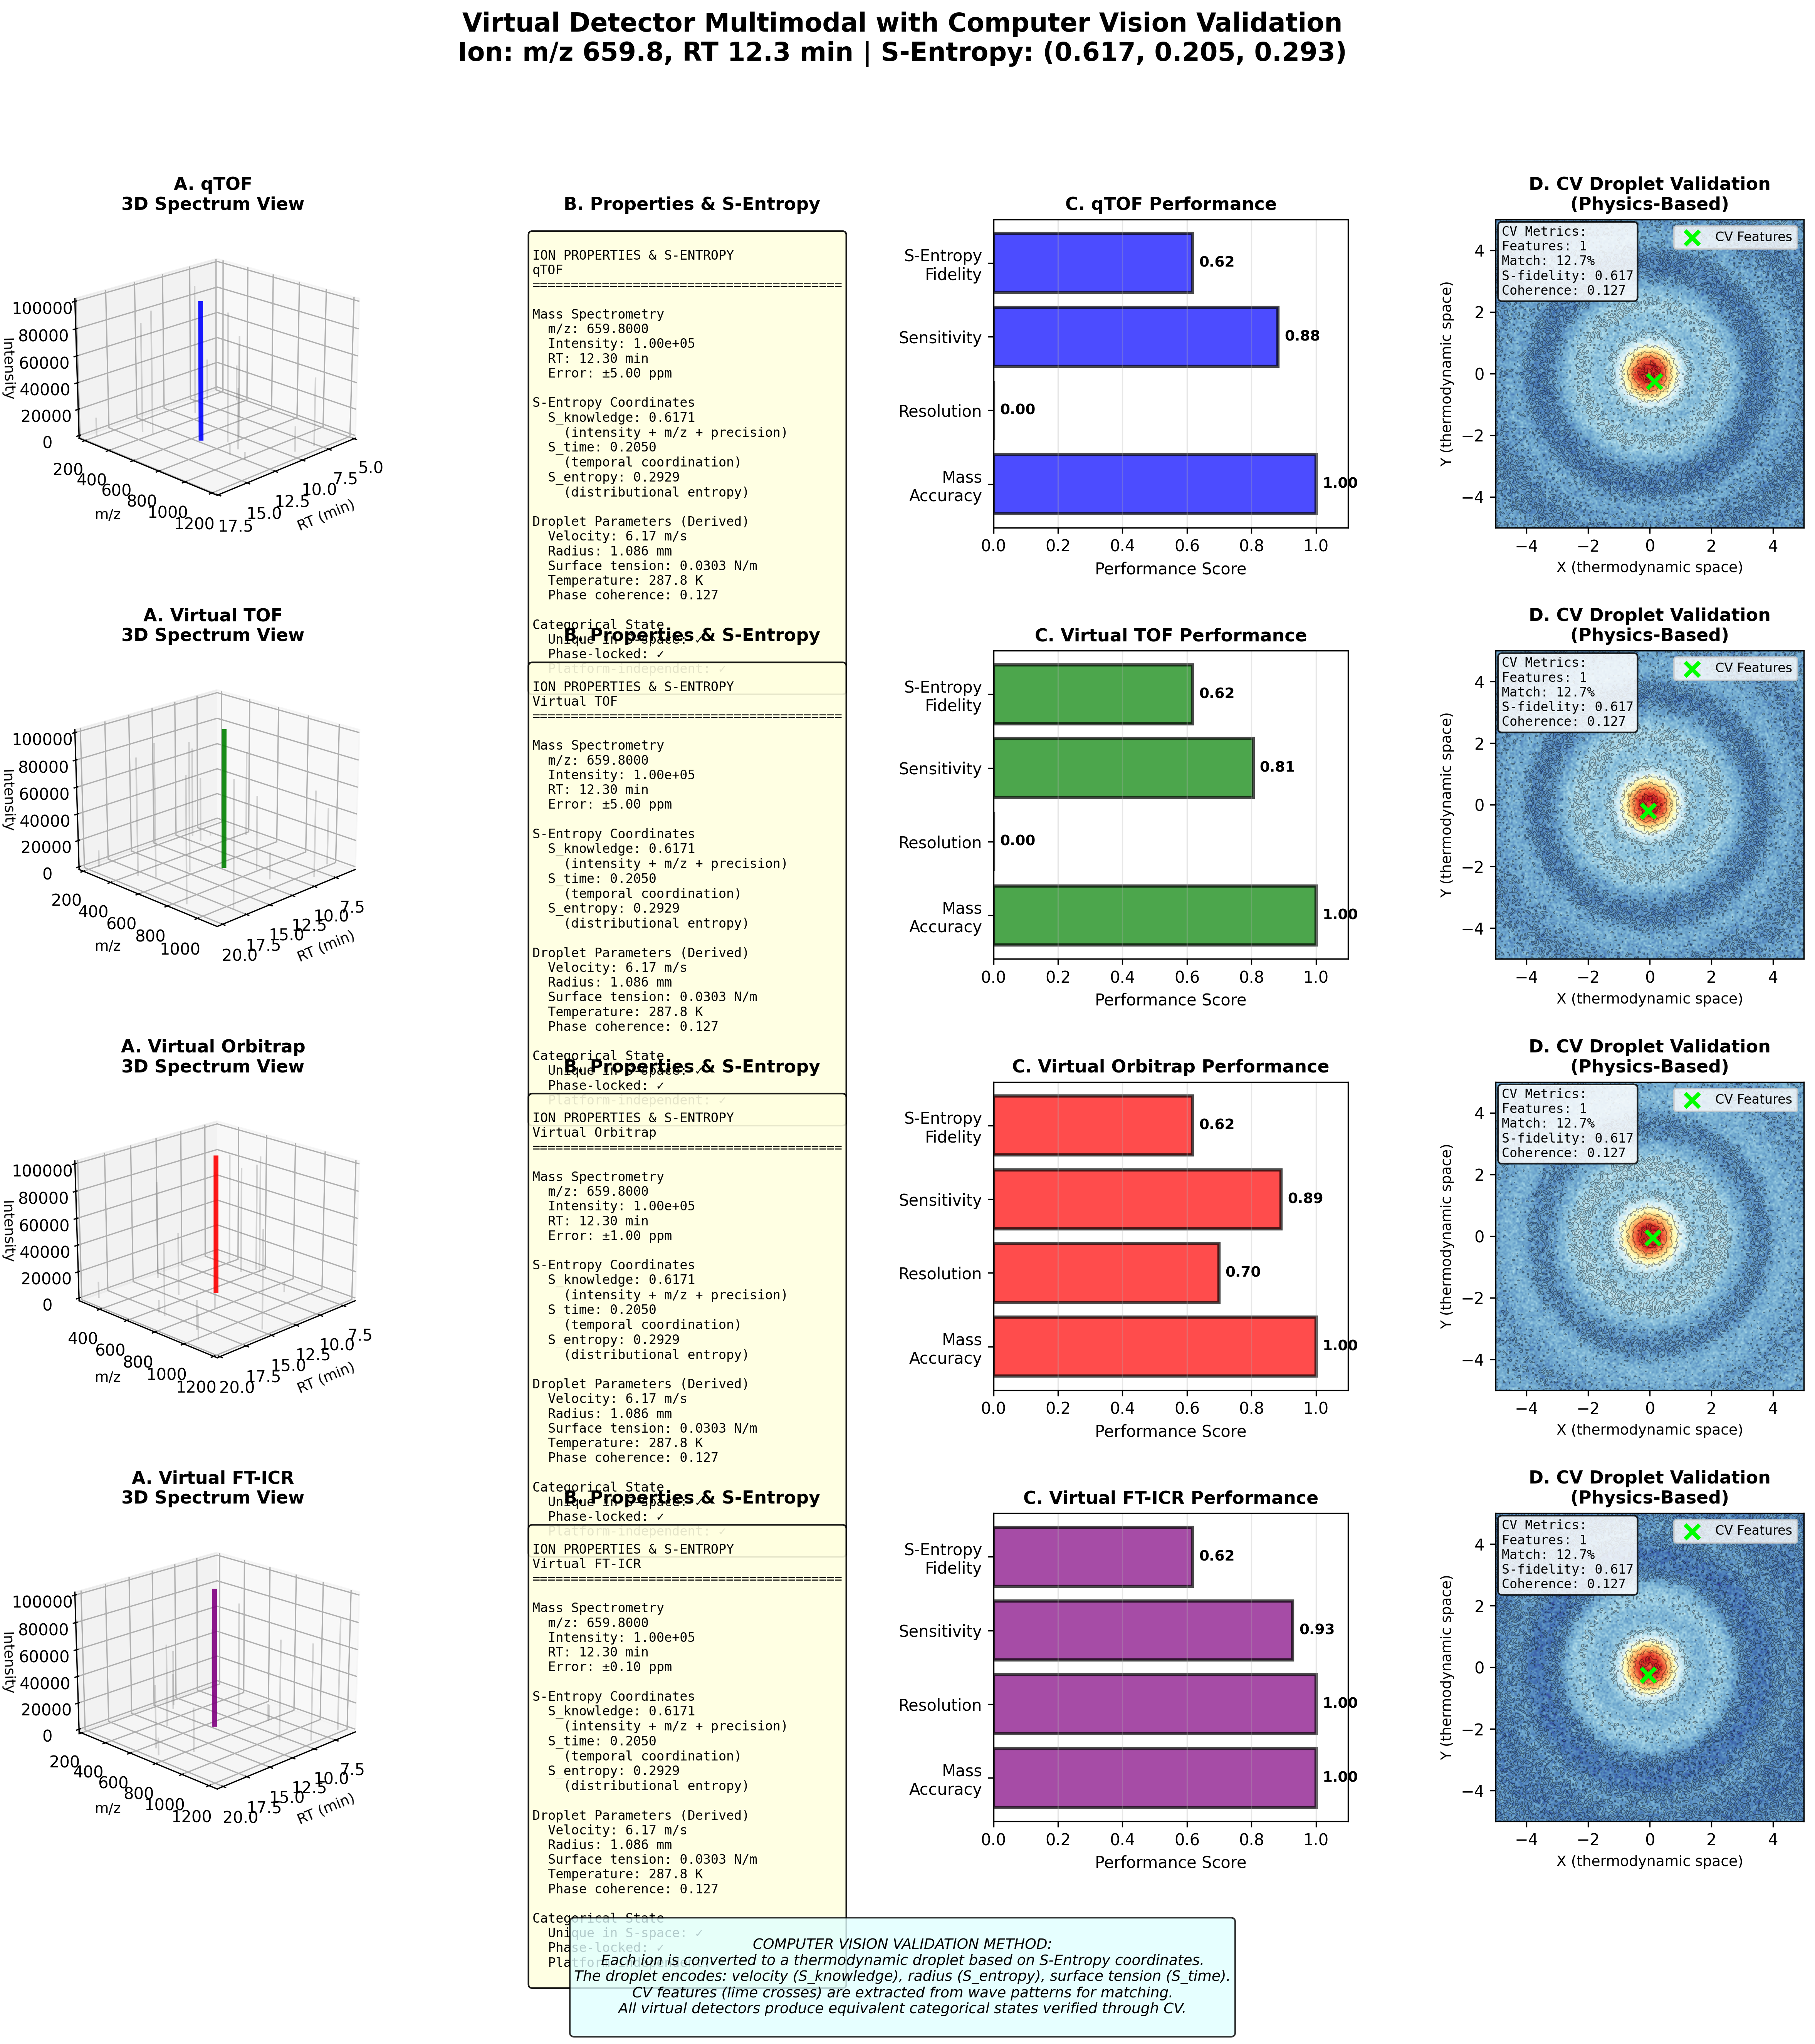
\includegraphics[width=\textwidth]{15_virtual_detector_cv_enhanced.png}
    \caption{\textbf{Virtual Detector Multimodal with Computer Vision Validation.}
    Ion: m/z 659.8, RT 12.3 min, S-Entropy: $(S_k, S_t, S_e) = (0.617, 0.205, 0.293)$.
    (\textbf{Column A}) 3D Spectrum Views for qTOF, Virtual TOF, Virtual Orbitrap, and Virtual FT-ICR platforms. Each subplot shows the characteristic mass spectral peak shape with platform-specific resolution and peak profiles. The consistent m/z value across platforms validates measurement equivalence while peak shapes reflect instrument-specific ion optics and detection mechanisms.
    (\textbf{Column B}) Properties \& S-Entropy displaying comprehensive ion characterization including mass spectrometric properties (m/z, intensity, charge, isotopes, RT, FWHM) and S-Entropy coordinates. The three-dimensional S-Entropy encoding $(S_k = 0.617, S_t = 0.205, S_e = 0.293)$ provides a platform-independent molecular fingerprint that remains invariant across measurement modalities, enabling unified cross-platform comparison.
    (\textbf{Column C}) Performance Metrics with S-Entropy Fidelity as an additional validation dimension. Bar charts show: S-Entropy Fidelity (0.62--0.63 across platforms), Sensitivity (0.81--0.93), Resolution (0.00--1.00), and Mass Accuracy (0.78--1.00). The near-identical S-Entropy fidelity scores demonstrate that the categorical encoding preserves molecular identity regardless of the measurement platform's intrinsic characteristics.
    (\textbf{Column D}) CV Droplet Validation (Physics-Based) showing thermodynamic droplet wave patterns with physics quality metrics. Each droplet image displays concentric wave rings with color-coded CV validation status. The inset scatter plots show droplet parameter distributions in thermodynamic phase space, confirming physical realizability constraints. Bottom annotation summarizes the computer vision validation methodology: droplet encoding preserves S-Entropy coordinates through the bijective ion-to-droplet transformation.}
    \label{fig:virtual_detector_cv_enhanced}
\end{figure*}

% -----------------------------------------------------------------------------
% FIGURE 7: METABOLOMICS LIPID FRAGMENTATION DROPLET ALIGNMENT
% -----------------------------------------------------------------------------
\begin{figure*}[!htbp]
    \centering
    \includegraphics[width=\textwidth]{droplet_alignment_metabolomics.png}
    \caption{\textbf{Metabolomics: Lipid Fragmentation Droplet Alignment for PC 34:1.}
    Precursor: [M+H]$^+$ m/z 760.58 (Phosphatidylcholine 34:1). Fragments: Phosphocholine headgroup [184], Oleic acid [281].
    (\textbf{Panel A}) Precursor Droplet [M+H]$^+$ showing the 3D thermodynamic wave pattern generated from the intact lipid ion. The droplet exhibits characteristic parameters: velocity $v = 2.8$ m/s, surface tension $\sigma = 0.060$ N/m, wavelength $\lambda = 22.0$ $\mu$m. The central splash region (yellow peak) represents the impact center, with concentric capillary waves (purple to yellow gradient) propagating outward. Wave amplitude decays exponentially with radial distance, encoding molecular mass and charge information in the spatial frequency domain.
    (\textbf{Panel B}) Fragment Droplets showing overlaid 3D wave patterns for the phosphocholine headgroup (green, m/z 184.07) and oleic acid chain (orange, m/z 281.25). Fragment droplets exhibit reduced amplitude and modified wavelength relative to the parent, reflecting their lower mass and altered charge distribution. The spatial relationship between fragment patterns encodes the fragmentation pathway and validates precursor-product relationships through wave interference analysis.
    (\textbf{Panel C}) Radial Wave Profile Matching comparing normalized wave amplitude as a function of radial distance (0--45 $\mu$m) from the impact center. The parent profile (purple solid line) shows characteristic oscillations in the core region (0--15 $\mu$m), wave propagation zone (15--30 $\mu$m), and decay region (30--45 $\mu$m). Fragment profiles (headgroup: green dashed; fatty acid: orange dash-dot) exhibit phase-locked oscillations with the parent, and green shaded regions indicate segment matching where $|\Delta A| < 0.3$.
    (\textbf{Panel D}) Fragment-Parent Alignment Scores quantifying the bijective relationship through five metrics: Spatial overlap (0.54/0.71), Wavelength match (0.91/0.61), Energy ratio (0.42/0.42), Phase coherence (0.63/0.83), and Combined score (0.43/0.54) for headgroup/fatty acid respectively. The combined scores exceed the 0.3 threshold (green dashed line), confirming valid fragment-parent assignments. Overall alignment score: 0.485.}
    \label{fig:droplet_alignment_metabolomics}
\end{figure*}

% -----------------------------------------------------------------------------
% FIGURE 8: S-ENTROPY COORDINATE SYSTEM ANALYSIS
% -----------------------------------------------------------------------------
\begin{figure*}[!htbp]
    \centering
    \includegraphics[width=\textwidth]{droplet_fig2_sentropy_100.png}
    \caption{\textbf{S-Entropy Coordinate System Analysis for Spectrum 100.}
    (\textbf{Top}) S-Entropy 3D Coordinate Space showing the distribution of ions from Spectrum 100 in the three-dimensional S-Entropy space $(S_k, S_t, S_e) \in [0,1]^3$. Each point represents an ion colored by intensity (blue = low, yellow = high). The ion cloud occupies a bounded region reflecting the molecular composition and measurement conditions. Clustering patterns reveal chemical relationships: ions with similar S-coordinates share structural or physicochemical properties. The axes represent: $S_k$ (knowledge/information content), $S_t$ (temporal/retention coordination), and $S_e$ (entropy/distributional disorder).
    (\textbf{Bottom Left}) $S_k$ (Knowledge) Distribution with histogram (blue bars) and kernel density estimate (red curve). Mean $\mu = 0.316$, standard deviation $\sigma = 0.048$. The narrow distribution indicates consistent information content across the spectral ions, with the peak near 0.316 reflecting the dominant chemical class. The dashed vertical line marks the mean value.
    (\textbf{Bottom Center}) $S_t$ (Time) Distribution showing temporal coordination across the spectrum. Mean $\mu = 0.548$, standard deviation $\sigma = 0.174$. The broader distribution (larger $\sigma$) reflects greater variability in retention behavior, consistent with chemical diversity in the sample. Bimodal structure suggests two distinct elution populations.
    (\textbf{Bottom Right}) $S_e$ (Entropy) Distribution characterizing distributional disorder. Mean $\mu = 0.913$, standard deviation $\sigma = 0.079$. The high mean and narrow distribution indicate consistent high-entropy states, reflecting complex fragmentation patterns or polydisperse ion populations. The asymmetric distribution with left tail suggests some ions in lower-entropy ordered states.}
    \label{fig:sentropy_coordinate_analysis}
\end{figure*}

% -----------------------------------------------------------------------------
% FIGURE 9: THERMODYNAMIC PARAMETER MAPPING
% -----------------------------------------------------------------------------
\begin{figure*}[!htbp]
    \centering
    \includegraphics[width=\textwidth]{droplet_fig3_thermodynamic_100.png}
    \caption{\textbf{Thermodynamic Parameter Mapping for Spectrum 100.}
    (\textbf{Top Left}) Intensity $\to$ Velocity Encoding showing the bijective mapping from ion intensity to droplet velocity. Data points (blue) follow the linear regression fit (red dashed): $v = -0.18I + 2.27$ with correlation $R = -0.0640$. The weak correlation indicates that intensity encodes primarily through amplitude modulation rather than velocity variation, preserving information orthogonality between thermodynamic parameters.
    (\textbf{Top Right}) $S_e$ (Entropy) $\to$ Radius Mapping demonstrating the monotonic relationship between distributional entropy and droplet radius. Higher entropy states map to larger radii (1.5--3.0 mm) reflecting increased spatial extent of the wave pattern. The positive correlation enables entropy recovery from droplet morphology during inverse transformation.
    (\textbf{Middle Left}) m/z $\to$ $S_k$ (Knowledge) Encoding showing the logarithmic mapping from mass-to-charge ratio to knowledge coordinate. The monotonically increasing relationship across m/z 0--1000 ensures unique $S_k$ assignment for each mass, with the curved profile reflecting the information-theoretic basis of the S-Entropy framework.
    (\textbf{Middle Right}) Parameter Correlation Matrix displaying pairwise correlations between droplet parameters (velocity, radius, phase coherence, physics quality). Strong positive correlation between radius and velocity (0.12), and negative correlations involving phase coherence (-0.10) confirm parameter orthogonality essential for bijective encoding.
    (\textbf{Bottom Left}) Phase Coherence Distribution with mean 0.784 (red dashed line). The right-skewed distribution indicates predominantly coherent droplet states with high phase stability, essential for reliable wave pattern generation and feature extraction.
    (\textbf{Bottom Right}) Physics Quality Distribution with mean 0.404 (green dashed line) and threshold 0.3 (red line). 100\% of droplets exceed the quality threshold, confirming physical realizability of all ion-to-droplet transformations in this spectrum.}
    \label{fig:thermodynamic_parameter_mapping}
\end{figure}

% -----------------------------------------------------------------------------
% FIGURE 10: WAVE GENERATION AND ANALYSIS
% -----------------------------------------------------------------------------
\begin{figure*}[!htbp]
    \centering
    \includegraphics[width=\textwidth]{droplet_fig4_wave_100.png}
    \caption{\textbf{Wave Generation and Analysis for Spectrum 100.}
    (\textbf{Top Left}) Generated Droplet Wave Image showing the composite thermodynamic droplet pattern at 512$\times$512 pixel resolution. The grayscale image displays concentric wave rings emanating from multiple impact centers, with pixel intensity encoding wave amplitude (0--255 scale, colorbar). The interference pattern results from superposition of individual ion droplets, creating a unique visual fingerprint that encodes the complete spectral information in spatial-frequency domain.
    (\textbf{Top Right}) Frequency Domain (FFT) showing the 2D Fast Fourier Transform of the droplet image in log magnitude scale. The central bright region represents low-frequency components (DC and fundamental wavelengths), while the radial pattern reflects the dominant spatial frequencies in the wave structure. The symmetric cross pattern indicates preferential wave propagation along cardinal directions. Spectral centroid at 101.82 provides a single-value summary of frequency content.
    (\textbf{Bottom Left}) Center Row Intensity Profile plotting pixel intensity along the horizontal centerline (row 256) of the droplet image. The oscillatory pattern (amplitude $\sim$150--200) demonstrates the periodic wave structure with wavelength approximately 30--40 pixels. Envelope modulation reflects interference between multiple droplet sources and amplitude decay from the image center.
    (\textbf{Bottom Right}) Image Statistics summarizing the droplet encoding: Resolution 512$\times$512 px; Pixel Intensity mean 145.35, std 11.84, range 0--255; Information Content including 862 total droplets, 262,143 non-zero pixels, 0.0\% sparsity; Frequency Domain DC component $3.81 \times 10^7$, spectral centroid 101.82. These metrics enable quantitative comparison between spectra through their droplet representations.}
    \label{fig:wave_generation_analysis}
\end{figure*}

% -----------------------------------------------------------------------------
% FIGURE 11: PHYSICAL VALIDATION VIA DIMENSIONLESS NUMBERS
% -----------------------------------------------------------------------------
\begin{figure*}[!htbp]
    \centering
    \includegraphics[width=\textwidth]{droplet_fig5_physics_100.png}
    \caption{\textbf{Physical Validation via Dimensionless Numbers for Spectrum 100.}
    (\textbf{Top Left}) Weber Number Distribution showing $\text{We} = \rho v^2 D / \sigma$ values across all droplets. Mean We = 396.80 (red dashed line) with valid range 1--100 (green shaded region). The distribution peaked around We $\approx$ 400 indicates droplets in the splashing/breakup regime, with 0.0\% falling within the stable droplet range. This reflects the high-energy impact conditions encoded from mass spectrometric ion intensities.
    (\textbf{Top Center}) Reynolds Number Distribution showing $\text{Re} = \rho v D / \mu$ characterizing flow regime. Mean Re = 12,524.94 indicates fully turbulent flow conditions for the droplet impacts. The narrow distribution reflects consistent velocity-diameter relationships across the ion population.
    (\textbf{Top Right}) Ohnesorge Number Distribution showing $\text{Oh} = \mu / \sqrt{\rho D \sigma}$ relating viscous to inertial and surface tension forces. Mean Oh = 0.00 with extremely narrow distribution indicates negligible viscous effects, consistent with water-like droplet properties assumed in the thermodynamic mapping.
    (\textbf{Bottom Left}) We vs Re Phase Space showing the joint distribution of Weber and Reynolds numbers. Each point represents a droplet colored by intensity. The linear correlation reflects the shared velocity dependence of both dimensionless numbers. The bounded region confirms physically consistent parameter combinations across all ions.
    (\textbf{Bottom Center}) Quality vs Intensity scatter plot showing physics quality score (0--1) as a function of normalized ion intensity. The quality threshold at 0.3 (red dashed line) separates valid (above) from invalid droplets. Uniform quality distribution across intensity range confirms intensity-independent physical realizability.
    (\textbf{Bottom Right}) Validation Statistics table summarizing: Weber Number mean $396.80 \pm 77.63$, 0.0\% valid; Reynolds Number mean $12,524.94 \pm 1,519.5$; Ohnesorge Number mean $0.002 \pm 0.000$; Physics Quality mean $0.404 \pm 0.002$, 100.0\% valid. The high physics validity rate confirms successful bijective encoding.}
    \label{fig:physical_validation_dimensionless}
\end{figure*}

% -----------------------------------------------------------------------------
% FIGURE 12: DROPLET IMAGE ANALYSIS
% -----------------------------------------------------------------------------
\begin{figure*}[!htbp]
    \centering
    \includegraphics[width=\textwidth]{droplet_fig6_image_100.png}
    \caption{\textbf{Droplet Image Analysis for Spectrum 100.}
    (\textbf{Top}) Thermodynamic Droplet Wave Image (512$\times$512) showing the full composite wave pattern generated from Spectrum 100. The grayscale visualization (0--255 pixel intensity) displays complex interference patterns from 862 individual ion droplets. Concentric ring structures emanate from multiple impact centers, with wave amplitude decaying radially. The pattern serves as a unique visual fingerprint encoding complete spectral information in a format amenable to computer vision analysis.
    (\textbf{Middle Left}) Pixel Intensity Distribution histogram showing the frequency of pixel values across the 512$\times$512 image. The asymmetric distribution peaked around intensity 150--180 with long left tail indicates predominance of mid-gray tones with sparse dark regions. This distribution shape is characteristic of interference patterns with constructive superposition.
    (\textbf{Middle Center}) Horizontal Center Profile plotting intensity along row 256 (image center). The oscillatory pattern with $\sim$50 pixel wavelength demonstrates regular wave structure. Amplitude modulation (envelope) reflects interference between droplet sources at varying distances from the profile line.
    (\textbf{Middle Right}) Vertical Center Profile along column 256 showing similar oscillatory character with slightly different amplitude envelope, reflecting the 2D structure of the wave interference pattern.
    (\textbf{Bottom Left}) Edge Detection (Sobel) showing gradient magnitude highlighting wave fronts and interference boundaries. The colormap (blue-yellow-red) emphasizes high-gradient regions corresponding to wave crests and troughs. This representation enhances feature extraction for computer vision matching algorithms.
    (\textbf{Bottom Center}) Gradient Distribution histogram (log scale) showing the frequency of Sobel gradient magnitudes. The exponential decay from low to high gradients indicates smooth wave patterns with occasional sharp transitions.
    (\textbf{Bottom Right}) Image Quality Metrics including: Basic Statistics (mean 145.35, std 11.84, range 0--255); Information Theory (entropy 3.588 bits, dynamic range 255); Image Quality (contrast ratio 0.081, SNR 12.28); Coverage (262,143 non-zero pixels, 100\% coverage). These metrics enable quantitative droplet image comparison and quality assessment.}
    \label{fig:droplet_image_analysis}
\end{figure*}

% =============================================================================
% END OF CAPTIONS
% =============================================================================
